\documentclass[11pt,letterpaper]{article}
\usepackage{array}
\usepackage{fullpage}
\usepackage{graphicx}
\usepackage{parskip}
\usepackage{amsmath}
\usepackage[small]{caption}
\usepackage{graphpap}
\usepackage{logpap}
\usepackage{tabularx}
\usepackage{url}
\usepackage{hyperref}
\usepackage{enumitem}

\renewcommand{\thesection}{PART \arabic{section}: }

\newcounter{question}[section]
\newenvironment{question}[1][]{\refstepcounter{question}\par\medskip
   \textbf{\arabic{section}.\thequestion.} \rmfamily}{\medskip}

\usepackage{titlesec}
\titleformat{\section}{\clearpage\normalfont\bfseries}{\thesection}{0em}{}
\titlespacing{\section}{0pt}{0.5\baselineskip}{0pt}

\titleformat{\subsection}[runin]
{\normalfont\bfseries}{\thesubsection}{1em}{}

\titleformat{\subsubsection}{\normalfont\bfseries}{\thesubsubsection}{0em}{}
\titlespacing{\subsubsection}{0pt}{0.5\baselineskip}{0pt}

\newcounter{saveenumi}
\newcommand{\seti}{\setcounter{saveenumi}{\value{enumi}}}
\newcommand{\conti}{\setcounter{enumi}{\value{saveenumi}}}

\usepackage[dvipsnames]{xcolor}
\newcommand{\sol}[1]{{\color{NavyBlue} #1}}



\begin{document}
\setlength{\parindent}{0in}

%% EQUIP: Force Probe, Pulley, Track, Hangar, Weight, Tilt, Scale

\begin{flushright}
PHYS S211: General Physics I\\
Lab 4: Circular Motion\\
10/1/24 (due 10/8/24)
\end{flushright}

Name:

\subsection*{Topics:}
\begin{enumerate}
\setlength{\parskip}{3pt}
\item Uniform circular motion
\item Centripetal acceleration
\end{enumerate}

\subsection*{Introduction:}
In this lab you will explore uniform circular motion and centripetal acceleration. The lab consists of several related exercises, each designed to isolate different variables related to circular motion. 

%{\bf Introduction:}\\
%If an object travels in a circular path with constant speed, the direction of its velocity is continuously changing; the object must therefore be continuously accelerating. This acceleration is referred to as the centripetal (or center-seeking) acceleration. The centripetal acceleration points inward along the radius that connects the object with the center of its circular path. For a path of radius $r$ and linear speed $v$, the centripetal accceleration $a_c$ is given by
%$$a_c = \frac{v^2}{r}.$$

%From Newton's second law, we know that the magnitude of the centripetal force $F_c$, necessary for this centripetal acceleration on a body of mass $m$ is
%$$F_c = ma_c = \frac{mv^2}{r}.$$

%Note that this force arises when an object pushes or pulls on the travelling object. In this lab the centripetal force will be due to the tension in a string. There is nothing special about a centripetal force; it carries a special name for historical reasons only. This lab is designed to test this equation experimentally and can therefore be regarded as another experimental test of Newton's laws.

%{\bf Procedure:}\\
Start by assembling an apparatus similar to the one shown in Figures \ref{fig:whirlingmass} and \ref{fig:whirlingmass2}. Mass $m_a$ on the order of 20 grams and a total string length of about 1.5 meters are good starting values. Attach mass $m_b$, which should be larger than $m_a$, to the string and tie mass $m_a$ {\bf securely} to the other end of the string; add a little bit of tape to help secure the knot.  In order for this to work, $m_b$ should be greater than $m_a$. Move to an area where there is plenty of room and carefully whirl mass $m_a$ above your head.  You will find that mass $m_b$ moves up and down as the speed of rotation is changed.  With a little practice you can find a combination of angular speed, mass $m_b$, and radius of rotation that will place mass $m_b$ in equilibrium.  You should find it possible to keep the speed of rotation constant enough to keep mass $m_b$ stationary.

\begin{figure}[h]
\begin{center}
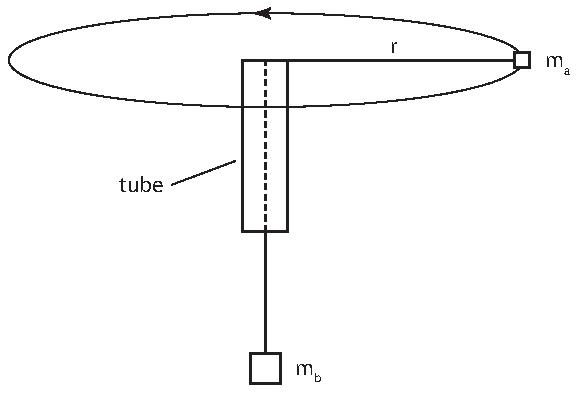
\includegraphics[scale=0.8]{./whirlingmass}
\end{center}
\caption{Diagram of a system in which masses $m_a$ and $m_b$ are connected by a string that is fed through a tube. Mass $m_a$ is whirled about the tube with an orbital radius of $r$. If the speed of rotation is too small, mass $m_b$ moves downward.  If the speed of rotation is too great, mass $m_b$ moves upward. %The  {\bf weight} (i.e., gravitational force) of mass $m_b$ provides the centripetal force that causes the velocity of mass $m_a$ to change direction.
}
\label{fig:whirlingmass}
\end{figure}

\begin{figure}[h]
\begin{center}
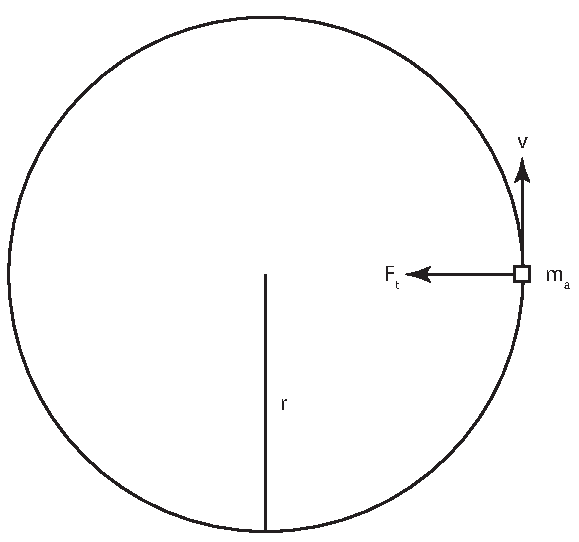
\includegraphics[scale=0.8]{./orbit}
\end{center}
\caption{Aerial view of mass $m_a$ moving in a circular path. The variables $m_a$, $r$, and $F_t$ can be chosen independently. The remaining variable, $v$, is measured indirectly. Be careful with units.}
\label{fig:whirlingmass2}
\end{figure} 



The goals of this lab are (1) to find empirical relationships between the mass, speed, and radius of the whirling mass and the tensional force in the string and (2) to compare the empirical relationship to theory.

\vspace{1cm}
\subsection*{What you should turn in:} A formal lab report. You are expected to write and submit an individual report, and you should submit it via Blackboard. The lab report should consist of the following parts:
\begin{itemize}
\item Introduction: Describe the topic/theory that you are exploring. Provide relevant background material. At the end of the introduction you should indicate in a brief statement or two how you will test that theory. (15 pts)
\item Methods: Describe the experimental set-up. Include a diagram if it clarifies your description. (15 pts)
\item Results: Present data, including qualitative descriptions, and graphs. Draw the reader's attention to
important aspects of the graphs. You should not discuss all of the minutiae of the data. All graphs should serve a purpose. If they aren't referenced in the text, don't include them. Avoid tables whenever possible; graphs are almost always preferred. Please include the graphs within the body of the report, and make sure they are clearly labeled. (30 pts)
\item Discussion and Conclusions: Summarize and interpret your results. Discuss whether or not your observations are consistent with theory, and explain why the differences might occur. Do not simply state that
there was experimental error. If there was experimental error, describe \textit{how} it affected your
calculations. In other words, can the experimental error actually explain the differences between your data and theory? Discuss how your assumptions may have affected your results. This will take some careful analysis of the problem that you are investigating. (25 pts)
\item Composition (not a separate section): Be sure that somebody that is unfamiliar with the lab exercise can understand what you've done. (15 pts)
\end{itemize}


A lab report does not need to be long to be good. You want your report to be thorough yet succinct. This takes practice. For additional tips on writing lab reports, see the information sheet  and rubric that I posted to Blackboard.\\





%Once you have found a combination of speed, radius, and mass that will keep mass $m_b$ in equilibrium, have your lab partner time you for some definite period of time (approximately 30 s) while you count the number of revolutions during this time interval.  Helpful hint: Make a mark on the string to help to you visually keep the radius constant. If you counted $N$ revolutions in time $T$, then the frequency is $N/T$.  Each revolution is $2 \pi $ in length, and so the linear speed of mass $m_a$ is given by $$v=2\pi{r}\frac{N}{T}.$$

%If $T$ is measured in seconds and $r$ in meters, then the speed will
%be in meters/second.  If masses $m_a$ and $m_b$ are determined in
%kilograms then the weight of mass $m_b$ and the centripetal force will
%be in Newtons.  
%\makeatletter
%\setlength{\@fptop}{0pt}
%\makeatother





\section{FORCE BALANCE EQUATIONS}
Using Figures 1 and 2 as a guide, use Newton's Second Law to write down an expression that relates the tensional force in the string to the mass, speed, and radius of the whirling mass. To perform these experiments, you will also need a couple of equations to calculate the speed of the whirling mass and the tension in the string. Use kinematics to write down an equation for determining the orbital velocity of the whirling mass, and Newton's First Law to determine how you can estimate the tensional force.

Include these equations, and a description of where they came from, in the introduction of your lab report.




\section{RELATIONSHIP BETWEEN FORCE AND SPEED}
%{\bf CAUTION: Mass $m_a$ will become a missile if the string breaks!}
\begin{enumerate}
\item Measure the mass $m_a$, which will be held constant for this part of the lab. $m_a=$

\item For this experiment you will vary $m_b$ and hold $r$ constant. Mark the string with a marker so that you can ensure that $r$ remains relatively constant. $r=$ 

Measure the period for each of several values of $m_b$. Calculate the speed and record your values in Table 1.
\end{enumerate}

\vspace{.5cm}

\newcolumntype{Y}{>{\centering\arraybackslash}X}%
%\begin{tabularx}{\linewidth}{|Y|Y|Y|Y|}
\begin{tabularx}{\linewidth}{|Y|Y|Y|Y|Y|}
\hline
$m_b$ & $F = m_b g$ & total time & \# of revolutions & $v$\\
%$r$ & $ F = m_B g$ & $m$ & $v$\\
\hline\vspace{2cm}&\vspace{2cm}&\vspace{2cm}&\vspace{2cm}&\vspace{2cm}\\
\vspace{2cm}&\vspace{2cm}&\vspace{2cm}&\vspace{2cm}&\vspace{2cm}\\
\hline\vspace{2cm}&\vspace{2cm}&\vspace{2cm}&\vspace{2cm}&\vspace{2cm}\\
\vspace{2cm}&\vspace{2cm}&\vspace{2cm}&\vspace{2cm}&\vspace{2cm}\\
\hline\vspace{2cm}&\vspace{2cm}&\vspace{2cm}&\vspace{2cm}&\vspace{2cm}\\
\vspace{2cm}&\vspace{2cm}&\vspace{2cm}&\vspace{2cm}&\vspace{2cm}\\
\hline\vspace{2cm}&\vspace{2cm}&\vspace{2cm}&\vspace{2cm}&\vspace{2cm}\\
\vspace{2cm}&\vspace{2cm}&\vspace{2cm}&\vspace{2cm}&\vspace{2cm}\\
%\hline\vspace{2cm}&\vspace{2cm}&\vspace{2cm}&\vspace{2cm}&\vspace{2cm}&\vspace{2cm}\\
%\vspace{2cm}&\vspace{2cm}&\vspace{2cm}&\vspace{2cm}&\vspace{2cm}&\vspace{2cm}\\
%\hline
%\hline\vspace{2cm}&\vspace{2cm}&\vspace{2cm}&\vspace{2cm}&\vspace{2cm}&\vspace{2cm}&\vspace{2cm}\\
%\vspace{2cm}&\vspace{2cm}&\vspace{2cm}&\vspace{2cm}&\vspace{2cm}&\vspace{2cm}&\vspace{2cm}\\
%\hline\vspace{2cm}&\vspace{2cm}&\vspace{2cm}&\vspace{2cm}&\vspace{2cm}&\vspace{2cm}&\vspace{2cm}\\
%\vspace{2cm}&\vspace{2cm}&\vspace{2cm}&\vspace{2cm}&\vspace{2cm}&\vspace{2cm}&\vspace{2cm}\\
\hline
\end{tabularx}\\

\begin{enumerate}
\setcounter{enumi}{3}
\item Plot a graph of $F$ vs. $v$ ($F$ is on the $y$-axis and $v$ is on the $x$-axis). Find a relationship between $F$ and $v$ from your graph.

\item Compare and discuss your experimental results with that predicted from the equation that you derived in Part 1. Plot the theoretical equation for $F(v)$ on the same graph.
\end{enumerate}



\section{RELATIONSHIP BETWEEN RADIUS AND SPEED}
\begin{enumerate}
\item Using the same value for $m_a$ as above, choose one value of $F$
    (or $m_b$) used in part A and find the speed $v$ for a few different values
    of $r$.\\ 
    $m_a=$\\
    
    $m_b=$\\
    
    $F=m_bg=$

\item Fill in the table.
\end{enumerate}

\vspace{.5cm}

\newcolumntype{Y}{>{\centering\arraybackslash}X}%
%\begin{tabularx}{\linewidth}{|Y|Y|Y|Y|}
\begin{tabularx}{\linewidth}{|Y|Y|Y|Y|}
\hline
$r$ & total time & \# of revolutions & $v$\\
%$r$ & $ F = m_B g$ & $m$ & $v$\\
\hline\vspace{2cm}&\vspace{2cm}&\vspace{2cm}&\vspace{2cm}\\
\vspace{2cm}&\vspace{2cm}&\vspace{2cm}&\vspace{2cm}\\
\hline\vspace{2cm}&\vspace{2cm}&\vspace{2cm}&\vspace{2cm}\\
\vspace{2cm}&\vspace{2cm}&\vspace{2cm}&\vspace{2cm}\\
\hline\vspace{2cm}&\vspace{2cm}&\vspace{2cm}&\vspace{2cm}\\
\vspace{2cm}&\vspace{2cm}&\vspace{2cm}&\vspace{2cm}\\
\hline\vspace{2cm}&\vspace{2cm}&\vspace{2cm}&\vspace{2cm}\\
\vspace{2cm}&\vspace{2cm}&\vspace{2cm}&\vspace{2cm}\\
\hline
\end{tabularx}\\

\begin{enumerate}
\setcounter{enumi}{2}
\item Plot a graph of $r$ vs. $v$ and find a relationship between $r$ and
    $v$ from your graph. As before, compare the results to the equation that you derived in Part 1 by plotting a theoretical curve of $r(v)$ on the same graph as your data.
\end{enumerate}



\section{RELATIONSHIP BETWEEN MASS AND VELOCITY}
\begin{enumerate}
\item Use a few different values for $m_a$ to find a relationship between
$m_a$ and $v$ in a similar manner to what you did in parts 1 and 2. Here, you will want to hold $m_b$ and $r$ constant.\\
$m_b=$\\

$F=m_bg=$\\

$r=$

\item Fill in the table below and plot $m_a$ vs $v$.
\end{enumerate}

\vspace{.5cm}

\newcolumntype{Y}{>{\centering\arraybackslash}X}%
%\begin{tabularx}{\linewidth}{|Y|Y|Y|Y|}
\begin{tabularx}{\linewidth}{|Y|Y|Y|Y|}
\hline
$m_a$ & total time & \# of revolutions & $v$\\
%$r$ & $ F = m_B g$ & $m$ & $v$\\
\hline\vspace{2cm}&\vspace{2cm}&\vspace{2cm}&\vspace{2cm}\\
\vspace{2cm}&\vspace{2cm}&\vspace{2cm}&\vspace{2cm}\\
\hline\vspace{2cm}&\vspace{2cm}&\vspace{2cm}&\vspace{2cm}\\
\vspace{2cm}&\vspace{2cm}&\vspace{2cm}&\vspace{2cm}\\
\hline\vspace{2cm}&\vspace{2cm}&\vspace{2cm}&\vspace{2cm}\\
\vspace{2cm}&\vspace{2cm}&\vspace{2cm}&\vspace{2cm}\\
\hline\vspace{2cm}&\vspace{2cm}&\vspace{2cm}&\vspace{2cm}\\
\vspace{2cm}&\vspace{2cm}&\vspace{2cm}&\vspace{2cm}\\
\hline
\end{tabularx}\\

\begin{enumerate}
\setcounter{enumi}{2}
\item Plot the theoretical relationship for $m_a(v)$ and compare it to your measurements.
\end{enumerate}

\section{RELATIONSHIP BETWEEN FORCE, RADIUS, AND VELOCITY}
%buy clickers
Using $m_a$ as in part 1, swing $m_a$ in a circle of radius approximately one
meter.  Hold the tube steady and pull down on the string, in
effect increasing $F$.  (Please don't jerk the string or exert too
much force; mass $m_a$ can become a dangerous missile!)  Do this several times
and describe in words the relationship between $F$, $r$, and $v$.  The
purpose of this section is two-fold.  First, it should give you a more literal feel for the centripetal force. Second, you should find it difficult to analyze the situation in which three quantities are simultaneously changing. This demonstrates why experimental technique is generally based on the idea of holding as many variables constant as possible. You do not need to make any measurements for this part of the lab but you should include a brief discussion (a few sentences) in your report.

\section{DISCUSSION OF ERROR}
There are at least two important sources of error in this lab. Identify the sources of error and (importantly!) describe in your report how the error affects your experiments. Are the sources of error random or systematic? Do the errors become larger when you change one of the variables? Why? 

%\clearpage
%\textbf{\MakeUppercase{Part 5: Discussion}}\\
%Use these questions to help guide your lab report.

%\begin{enumerate}
%\item How is the force on a rotating body affected by doubling the
%    radius while keeping the linear velocity constant?

%\vspace{3cm}

%\item A car travelling on a horizontal circular track has a constant
%    speedometer reading of 45 km/hr.  Is the car accelerating?  State
%    your reason(s) for your answer.  What exerts the force?

%\vspace{3cm}

%\item Sometimes it is stated that when a body is moved in a circular
%    path it is ``pushed outward by centrifugal force.''  Do you agree
%    with this statement?  Defend your answer.

%\vspace{3cm}

%\item Draw the free body diagram accompanying this experiment.

%\vspace{3cm}

%\item In addition to measurement errors, what other errors or assumptions are implicit in these lab exercises? How would you expect them to affect the results?
%\end{enumerate}

\end{document}
